\chapter{Introducción}
\label{capitulo1}
\lhead{Capítulo 1.}

% De qué va a tratar el capítulo
% El capítulo 1 suele ser el marco teórico.

\section{Objetivos}
\subsection{Objetivos generales}
El objetivo del presente trabajo es incorporar la técnica de detección de intrusiones SSM propuesta en [1] en el sistema Bro. Para ello deben usarse las capacidades de scripting de Bro e incorporar las funcionalidades necesarias como un módulo que pueda activarse a demanda para monitorizar las peticiones a los servicios web.
\subsection{Objetivos especificos}
La consecución del objetivo general planteado puede abordarse a partir de los siguientes objetivos específicos:

\begin{enumerate}
\item Interceptar las URI para su análisis haciendo uso de las herramientas presentadas por Bro para capturar y filtrar la información de los paquetes del protocolo HTTP.
\item Desarrollar un módulo que permita evaluar el índice de anomalía de los URI.
Se diseñará e implementará un módulo de evaluación haciendo uso de las herramientas otorgadas por el lenguaje de scripting de Bro y siguiendo las especificaciones y expresiones pautadas por la técnica de detección de intrusiones SSM. 
\item Desarrollar un módulo para la estimación de los modelos de normalidad
Se diseñará e implementará un módulo de entrenamiento haciendo uso de las herramientas otorgadas por el lenguaje de scripting de Bro que permita obtener un modelo de normalidad a partir de trafico libre de ataques.
\item Evaluar experimentalmente el funcionamiento del sistema
Se realizarán pruebas, tanto funcionales como operativas para verificar el correcto funcionamiento del sistema.
\end{enumerate}

\section{Planificación}

La tareas en las que se dividió el desarrollo de este proyecto fueron las siguientes:

\newlist{legal}{enumerate}{10}
\setlist[legal]{label*=\arabic*.}

\begin{legal}
\item Estado del arte
Durante esta etapa se realizó un estudio sobre los IDS, los tipos de IDS y el sistema SSM. Así mismo, se hizo una lectura del RFC 3986 (URI) y se investigó sobre el protocolo HTTP.

\item Análisis de Bro 
Durante esta etapa del proyecto se instaló, se estudio la documentación y se aprendió a hacer uso de la herramienta Bro y su lenguaje de scripting.

\item Arquitectura modular del sistema 

En esta etapa se realizó el diseño de los módulos principales que conforman el sistema. Esta tarea se basó en dividir el trabajo de cada uno de los módulos en varias funcionalidades y en diseñar las estructuras de datos y el formato de los archivos de texto del sistema.

    Esta tarea estuvo subdividida en las siguientes subtareas:

\begin{legal}
\item Diseño del módulo de análisis sintáctico/segmentación de URIS 
\item Diseño del módulo de evaluación de URIs 
\item Diseño del módulo de entrenamiento 
\end{legal}
\item Implementación del sistema 
En esta etapa del proyecto se llevó a cabo la implementación del sistema haciendo uso del lenguaje de scripting de Bro.

\begin{legal}
\item Módulo de análisis sintáctico/segmentación de URIS 

En esta etapa se tomaron los diseños esbozados previamente y se implementaron todas las funcionalidades necesarias para realizar el segmentador y el analizador sintáctico de los URIS. Fue necesario hacer uso de expresiones regulares y de las herramientas otorgadas por Bro para manejarlas.

\item Módulo de evaluación de URIs 

En esta etapa se tomaron los diseños realizados y se implementaron todas las expresiones, las estructuras de datos y las funcionalidades necesarias para construir un modulo de evaluacion funcional haciendo uso de las herramientas presentadas por Bro. 

\item Módulo de entrenamiento 

En esta etapa se implementaron las estructuras de datos y los dos modos de entrenamiento (Online y Offline) haciendo uso del lenguaje de scripting de Bro.

\item Módulo de gestión del tipo de modo del sistema
En esta etapa del proyecto se implementó el módulo de gestión del tipo de modo del sistema haciendo uso de bash scripting. Mediante este módulo se escogerá en que tipo de modo correrá el sistema (entrenamiento o evaluación).

\item Módulo de reportes
En esta etapa se implementaron los reportes del sistema haciendo uso de herramientas de Bro dedicadas exclusivamente a realizar este tipo de tareas.

\end{legal}
\item Evaluación y pruebas 
Una vez finalizada la implementación del sistema se procedió a realizar pruebas tanto funcionales como operativas.
\begin{legal}
\item Realización de pruebas funcionales

En esta etapa del proyecto se hicieron pruebas de manera individual a cada una de las funciones más importantes de los módulos que conforman el sistema y se realizaron las modificaciones adecuadas en las mismas.

\item Realización de pruebas operativas

La realización de las pruebas operativas se basó en tomar base de datos de trazas tanto normales como anormales, probar el funcionamiento de todo el sistema y realizar las modificaciones adecuadas.
\end{legal}

\item Documentación  
 Esta fase consistió en estructurar y redactar el libro del proyecto.
\end{legal}

A continuación, se mostrará un diagrama de Gantt en donde se muestra el tiempo que tomó cada una de las tareas.

\begin{center}
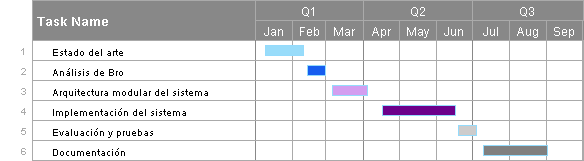
\includegraphics[width=4in]{Proyecto-grado.png}
\end{center}


\section{Presupuesto}

A continuación se mostrará una tabla que muestra el presupuesto del proyecto realizado.

\begin{center}
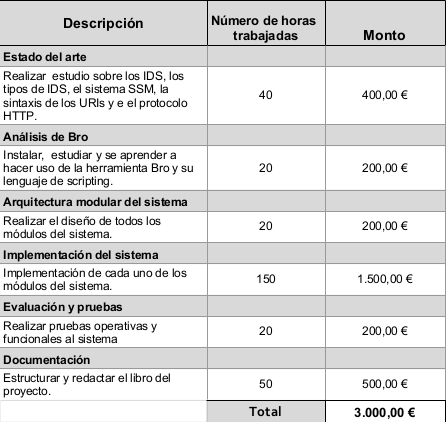
\includegraphics[width=4in]{presupuesto.png}
\end{center}